\section{Method}
\label{sec:method}
\begin{figure*}[t]
\centering
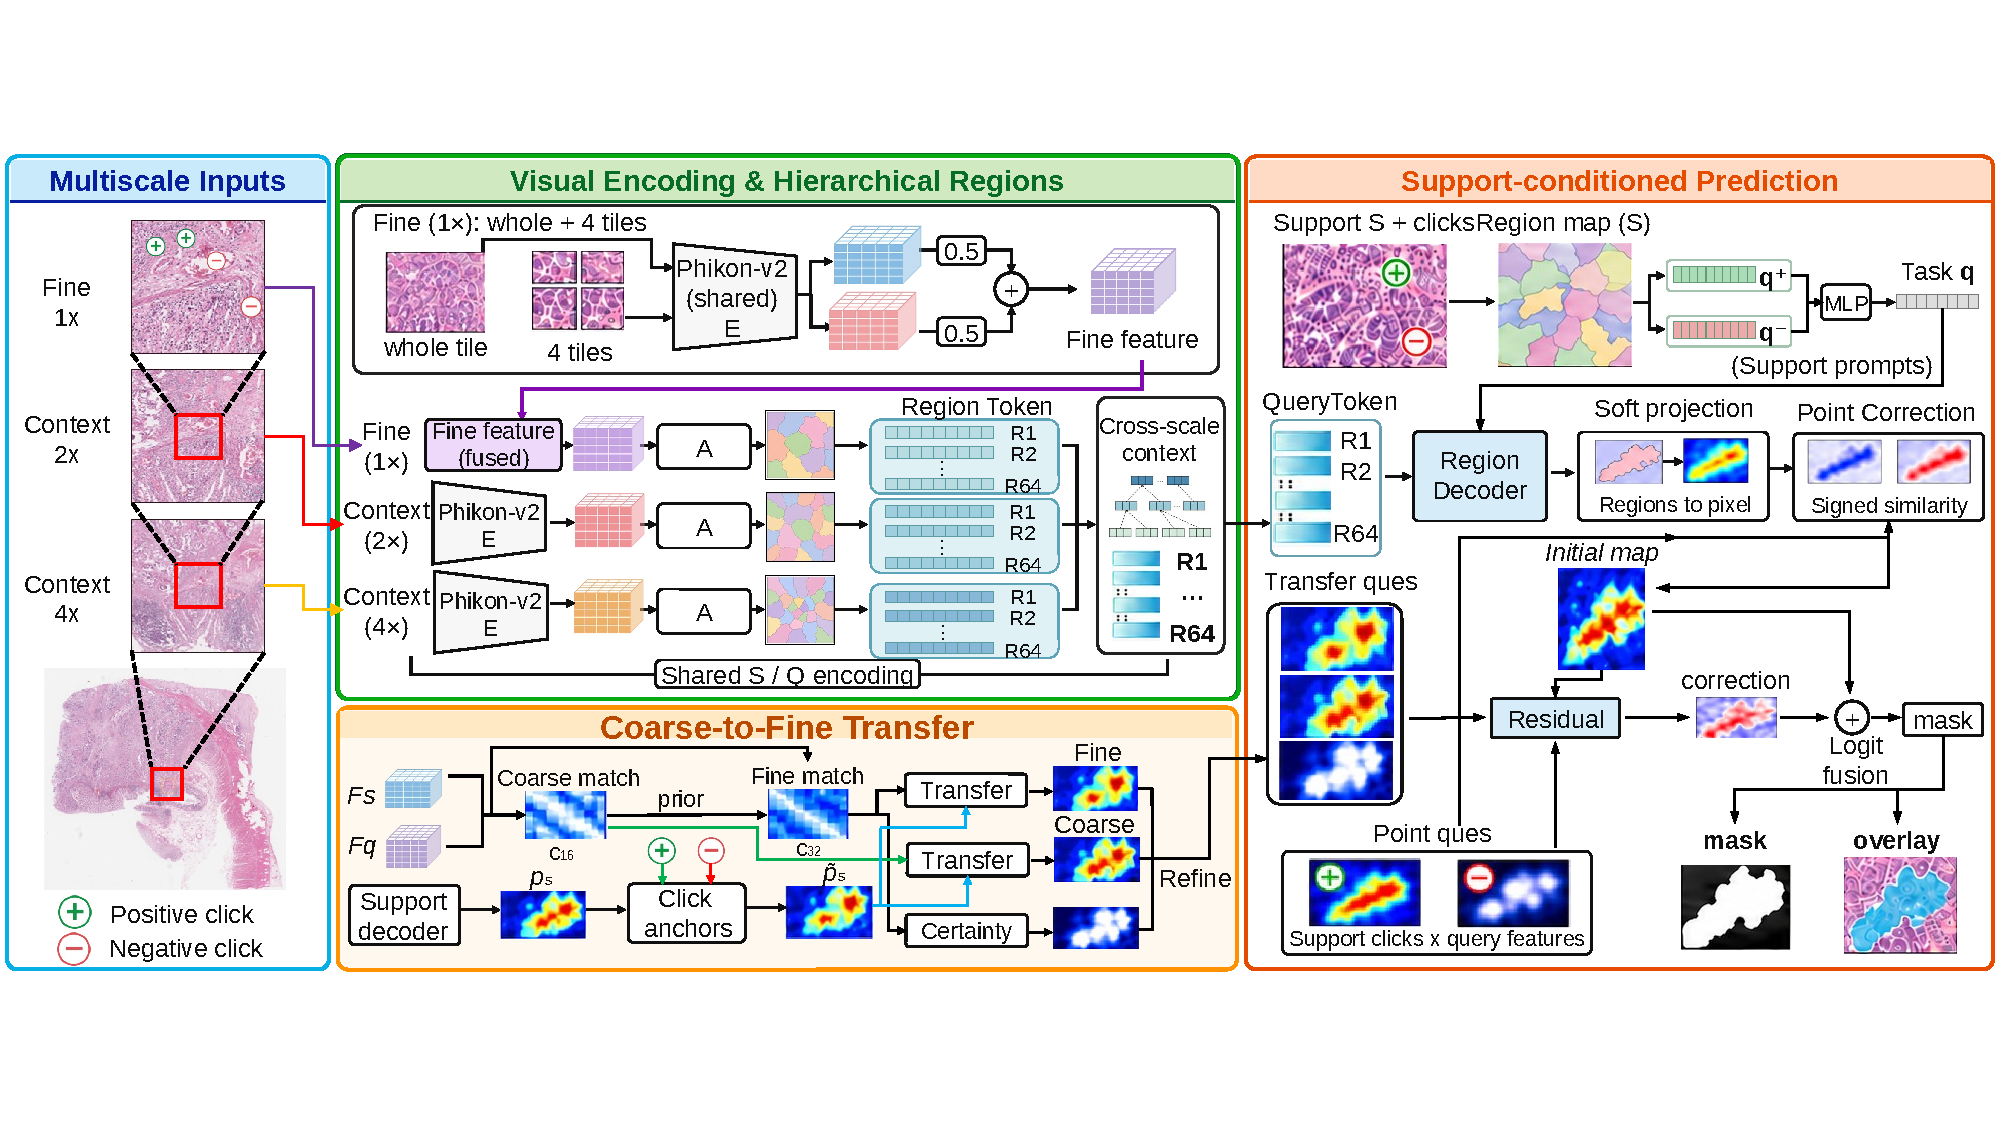
\includegraphics[width=\textwidth,trim=0 72bp 0 72bp,clip]{figures/method.pdf}
\caption{Overview of FewClick for same-slide support--query segmentation. Shared frozen Phikon-v2 features combine $1\times$, $2\times$, and $4\times$ views with whole/tiled fine-feature averaging. Soft assignments $A$ pool region tokens for cross-scale context exchange. Signed support clicks produce prompt summaries $q^+/q^-$ and task vector $q$ for query-region decoding. Soft projection and signed point-similarity correction yield $p_0$. The same path predicts support probabilities, which are click-anchored before transfer. Projected features $F_S/F_Q$ form coarse and prior-guided fine correspondences $C_{16}/C_{32}$; subscripts denote grid sizes. Transferred probabilities, entropy-based certainty, initial predictions, and point cues feed a bounded residual head. Its upsampled correction is added to the initial \emph{logits}, followed by sigmoid and thresholding at $0.5$. Remote queries receive no human clicks. Tissue inserts and intermediate maps are illustrative.}
\label{fig:overview}
\end{figure*}
FewClick propagates a click-defined tissue target across the same slide through signed support conditioning and dense probability transfer, using multiscale region context to organize spatial evidence (Fig.~\ref{fig:overview}).

\subsection{Prompt-Defined Tissue Segmentation}
Each interaction defines a binary target-versus-rest task. Let $W$ be a WSI, $S$ a support patch, $\mathcal P^+$ and $\mathcal P^-$ its positive and negative clicks, and $Q$ a query patch. We predict
\begin{equation}
 p_Q=f_\theta(Q\mid S,\mathcal P^+,\mathcal P^-).
\end{equation}
Support and remote query patches occupy different physical locations on the same slide. Remote patch evaluation requires their largest input footprints to be disjoint. A new slide or target receives a new support example. Training uses support and query annotations; inference uses their images and support clicks.

\subsection{Whole-Patch and Tiled Feature Fusion}
\label{sec:fusion}
Tissue architecture and fine structure require different sampling densities. For each support or query location, we extract concentric fine, $2\times$, and $4\times$ physical views and resize each to $512\times512$. All views use a shared, frozen public Phikon-v2 backbone.

The fine view has two encoding paths. One encodes the complete patch. The other divides it into four non-overlapping $256\times256$ tiles, resizes each tile to $512\times512$, and encodes its native $32\times32$ spatial tokens. Stitching the four grids restores their spatial arrangement at $64\times64$. We align the whole-patch grid to this resolution and fuse the two representations:
\begin{equation}
 E_f=\tfrac12\operatorname{Align}(F_{\rm whole})
     +\tfrac12\operatorname{Stitch}(F_1,F_2,F_3,F_4).
\label{eq:fusion}
\end{equation}
The larger views provide regional context. Each location requires seven backbone passes: one whole fine patch, four tiles, and two context views.

\subsection{Prompt-Conditioned Region Hierarchy}
\label{sec:regions}
\paragraph{Spatial context pooling.}
Each view forms $64$ region tokens of dimension $256$ on a $64\times64$ feature grid. Let $F_s(x)$ denote the projected backbone features at scale $s\in\{f,m,c\}$ and $a_s(x,k)$ the assignment-head output. Region $k$ has an anchor $c_k$ on a regular $8\times8$ grid. With positions $u(x)$ and anchors $c_k$ in $[-1,1]^2$, its soft assignment and pooled token are
\begin{align}
 A_s(x,k)&=\operatorname{softmax}_{k}\!\left(a_s(x,k)-\frac{\|u(x)-c_k\|^2}{0.08}\right),\label{eq:assignment}\\
 r_{s,k}&=\frac{\sum_x A_s(x,k)F_s(x)}{\max(\sum_x A_s(x,k),10^{-6})}.
\end{align}
The assignment head starts at zero and is updated by segmentation supervision. A shared fusion mapping processes the tokens using image features; auxiliary cell-context and count inputs are fixed to zero. Assignment regularization averages mass-balance, entropy, and compactness terms across views, with weights $0.01$, $0.001$, and $0.01$.

\paragraph{Cross-scale context.}
Physical overlap defines adjacent-scale connections. We map a child view into the central portion of its parent, accumulate overlap products between their assignment maps, and retain at most four valid parents per child region. This discrete edge construction is detached from the computation graph. Sparse bottom-up attention updates intermediate and then coarse tokens. Fine tokens receive top-down attention residuals from their parents and ancestors, gated by the hyperbolic tangent of a learned scalar initialized to zero. Region centers and areas are expressed in the common $4\times$ coordinate system.

\paragraph{Signed prompt encoding.}
We interpolate the fine assignment map at each support click and pool the corresponding region tokens. For set encoding, normalized tokens receive position, sign, and learned scale embeddings with a fixed scale index. Click coordinates lie in $[0,1]^2$. A shared two-layer, four-head set encoder~\cite{lee2019settransformer} and learned-query pooling separately summarize positive and negative sets into $q^+$ and $q^-$. Their contrast defines the task token:
\begin{equation}
 q=\operatorname{MLP}([q^+,q^-,q^+-q^-]).
\end{equation}

\paragraph{Region decoding and pixel projection.}
The $192$ region nodes receive scale embeddings. Query nodes cross-attend to support prompt tokens carrying position and sign embeddings and combine task, geometry, and signed cosine-similarity information. The graph decoder retains six-nearest-neighbor within-scale connections with self-loops and bidirectional adjacent-scale edges. A binary head predicts fine-region logits $o_k$. Upsampled, normalized assignments project region probabilities to pixels:
\begin{equation}
 p_r(x)=\sum_k\bar A_f(x,k)\,\sigma(o_k).
\label{eq:projection}
\end{equation}
We clip this probability to $[10^{-6},1-10^{-6}]$ before converting it to pixel logits. The same support-conditioned path also predicts the support mask.

\subsection{Signed Point-Similarity Correction}
\label{sec:point}
Regions encode context, while clicked locations provide direct appearance examples. A shared $1\times1$ projection maps the fine support and query features from $256$ to $64$ dimensions. We sample support features at the clicks and compute their cosine similarity to normalized query features.

The maximum and mean similarities for each sign, the difference of signed maxima, region probability $p_r$ resized to $64\times64$, and its uncertainty $4p_r(1-p_r)$ form seven input channels. A convolutional head predicts a correction, which is upsampled and added to the region-derived logits. Its final layer is zero-initialized. This path produces both the initial query probability $p_0$ and the support probability $p_S$.

\subsection{Coarse-to-Fine Dense Probability Transfer}
\label{sec:transfer}
We transfer the predicted support probability field through dense support--query correspondences.

\paragraph{Click-anchored support probabilities.}
Let $\bar p_S=\operatorname{Resize}_{32}(\operatorname{stopgrad}(p_S))$. Each field $g^+$ or $g^-$ sums unit-peak Gaussians over same-sign clicks, with standard deviation $1/32$ in $[0,1]^2$. The anchored probability is
\begin{equation}
 \widetilde p_S=\frac{\bar p_S+4g^+}{1+4g^++4g^-}.
\label{eq:anchor}
\end{equation}
This constrains the transferred support evidence near the clicks.

\paragraph{Coarse-to-fine correspondence.}
Average pooling converts the projected $64\times64$ features into $32\times32$ and $16\times16$ grids. After feature normalization, query--support cosine similarities form matrices $K_{32}$ and $K_{16}$. A softmax over support locations with temperature $\tau=0.1$ produces coarse correspondence $C_{16}$. Expansion $\mathcal U$ copies each coarse query row to its four child locations and divides each support location's mass among its four children. With $\Pi_{32}=\max(\mathcal U(C_{16}),10^{-8})$, we obtain
\begin{align}
 C_{16}&=\operatorname{softmax}_{S}(K_{16}/\tau),\\
 C_{32}&=\operatorname{softmax}_{S}\!\left(K_{32}/\tau
                  +0.5\log \Pi_{32}\right).
\label{eq:correspondence}
\end{align}
Rows index query locations and columns index support locations; $C_{16}$ and $C_{32}$ have sizes $256\times256$ and $1024\times1024$.

\paragraph{Transfer and residual refinement.}
Flattening probability grids into vectors, the correspondences transport the anchored field ($\operatorname{Pool}$ is $2\times2$ average pooling):
\begin{equation}
 t_{32}=C_{32}\widetilde p_S,\qquad
 t_{16}=C_{16}\operatorname{Pool}(\widetilde p_S).
\end{equation}
Transferred vectors are reshaped to their spatial grids. Matching certainty is one minus the entropy of each $C_{32}$ row divided by $\log 1024$. Fine transfer, resized coarse transfer, certainty, $p_0$, $4p_0(1-p_0)$, positive and negative maximum similarities, and their difference form eight channels $z_Q$ on the $32\times32$ grid. A $3\times3$ convolution, GELU, and $1\times1$ convolution predict a bounded logit residual:
\begin{equation}
 p_Q=\sigma\!\left(\operatorname{logit}(p_0)
                +\operatorname{Up}[2\tanh h(z_Q)]\right).
\label{eq:residual}
\end{equation}
Upsampling restores $512\times512$ output resolution. Dense transfer is used for remote tasks; local interaction uses the region and point-correction paths. The complete model retains both click anchoring and the coarse prior.

\subsection{Training Objective and Optimization}
\label{sec:training}
Training covers local interaction, same-slide target-present transfer, and target-absent transfer. The fixed queue contains $9{,}500$ tasks: $4{,}000$ local, $5{,}000$ remote target-present, and $500$ remote target-absent. Four tasks are accumulated per update, giving $2{,}375$ updates. The objective is
\begin{equation}
 \mathcal L=\mathcal L_Q+0.25\,\mathbf{1}_{\rm remote}\mathcal L_S
                  +0.1\mathcal L_{\rm click}+\mathcal L_{\rm assign}.
\end{equation}
Segmentation combines valid-pixel binary cross-entropy, soft Dice for target-present tasks, and boundary-band cross-entropy weighted by $0.5$. For target-absent queries, $0.1$ times the mean predicted probability replaces the Dice term. When both labels occur, cross-entropy averages the positive and negative pixel losses with equal weights. The click loss constrains support predictions at the signed prompts. $\mathcal L_{\rm assign}$ averages over support and query images for remote tasks.

We use AdamW with learning rate and weight decay both $10^{-4}$. The public backbone remains frozen, and downstream modules start from new initialization. Functional checks use training data, followed by fresh downstream initialization for formal training. Inference uses the final update and a fixed probability threshold of $0.5$.

\subsection{Whole-Slide Inference from One Support Set}
\label{sec:wsi}
Each slide--target pair receives one support patch and its signed clicks. Query windows reuse this support state; changing the slide or target resets it. With support fine-view dimensions $(b_w,b_h)$, the query grid uses strides $\lfloor b_w/2\rfloor$ and $\lfloor b_h/2\rfloor$. Edge-aligned windows complete the last row and column, and the support location is included. Context views stay concentric, with white padding outside the image.

Each window's probabilities are bilinearly mapped to the annotation grid using pixel-center alignment. At overlapping locations, we average all covering windows:
\begin{equation}
 p_W(x)=\frac{\sum_j\mathbf{1}[x\in\Omega_j]p_j(x)}
                   {\sum_j\mathbf{1}[x\in\Omega_j]},\qquad
 M_W(x)=\mathbf{1}[p_W(x)\geq0.5].
\end{equation}
Every output pixel must have at least one contribution. Full-slide Dice counts each valid annotated pixel once. Strict-remote evaluation removes the union of fine output rectangles from windows whose $4\times$ input footprints intersect the support's $4\times$ footprint. Predictions are fixed before annotations are read for scoring; unannotated pixels are excluded.
